

\chapter{协议设计}

\section{总体设计}

\subsection{基础代码源文件架构分析}
首先我们通过 tree 命令获得如图\ref{fig:structure}并绘制了项目结构的思维导图。

\begin{figure}[htbp!]
  \centering
  \subfigure[tree 指令得到的结构]{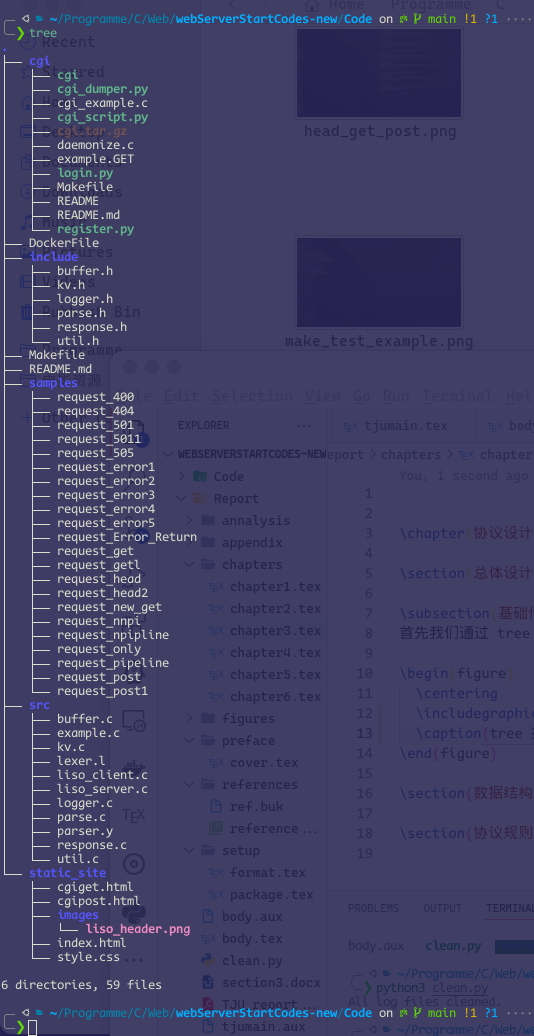
\includegraphics[width=1.624in]{Web_code_Structure.png}}
  \subfigure[文件结构的思维导图]{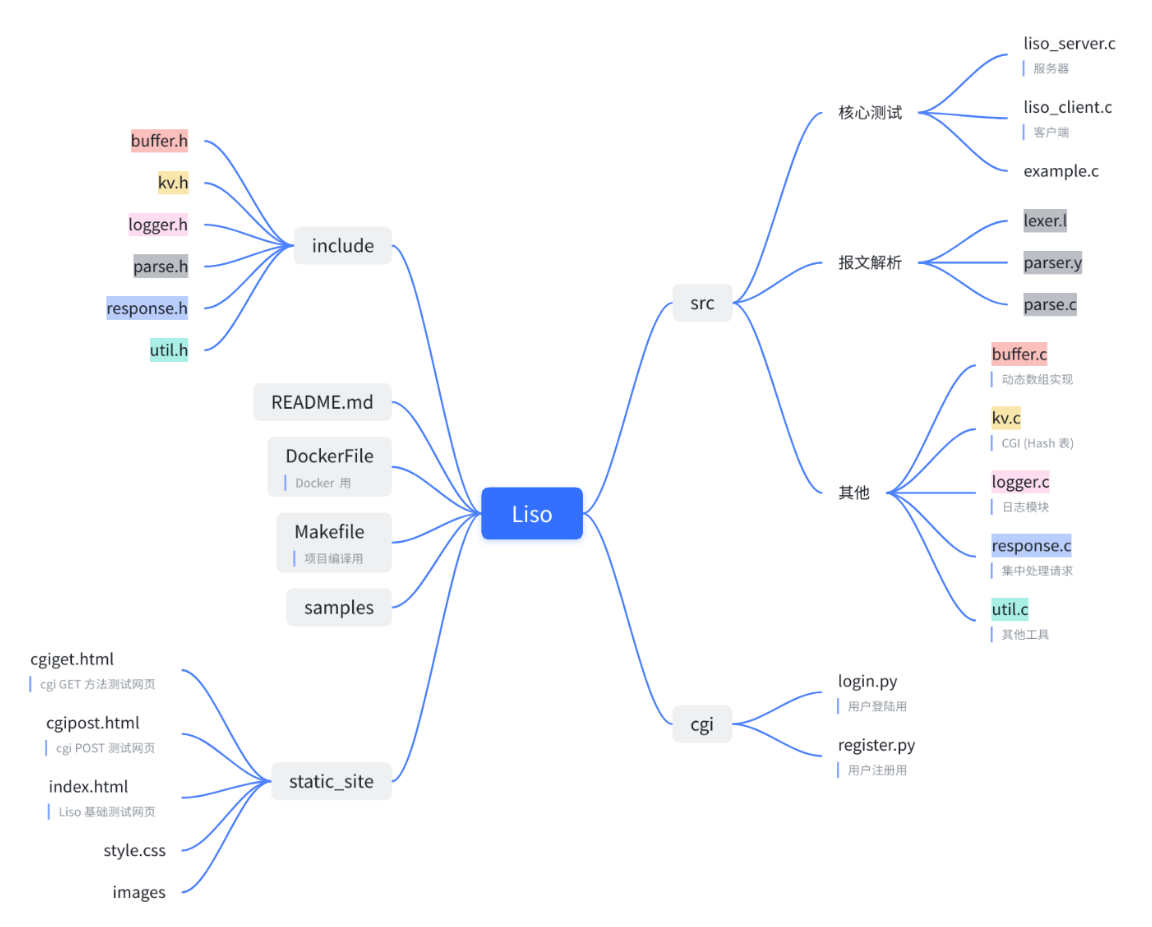
\includegraphics[width=4.1in]{Liso_structure.png}}
  \caption{项目文件结构}\label{fig:structure}
\end{figure}

可以看到,项目文件主要分为三大部分:静态网页、cgi 后端源码和服务器源码及其编译文件。三个部分是解耦和的,只需按照相应的接口进行测试,有相互依赖的问题。
其中,我们增加了诸如 buffer,kv,logger,response等文件,在表\ref{tab:structure} 中详细给出其用途及其类型。

\begin{table}[htbp!]
  \centering
  \begin{tabular}{p{5pt}p{65pt}p{220pt}p{60pt}}
  \hline
    & 文件                 & 用途描述         & 类型 \\ \hline
  1 & buffer.{[}c|h{]}   & 实现了 char* 数组增长、缩短、堆空间处理等功能的动态数组类型,用于处理缓冲区溢出问题 & 数据结构 \\
  2 & kv.{[}c|h{]}       & 实现了 CGI 环境变量、参数的数据结构,实现了键值对的添加以及堆空间的处理        & 数据结构\\
  3 & parse.{[}c|h{]}    & 处理报文解析   & 数据结构 \\
  4 & logger.{[}c|h{]}   & 实现了简单的日志管理工具 & 工具\\
  5 & response.{[}c|h{]} & 处理报文以及生成返回报文 & 函数集合 \\
  6 & util.{[}c|h{]}     & 其他小工具  & 工具宏 \\
  7 & login.py          & 用户登陆的 python 程序 & 后端程序\\
  8 & register.py       & 用户注册的 python 程序 & 后端程序\\
  9 & cgiget.html       & cgi METHOD 方法测试的网页 & 前端网页\\
  10 & cgipost.html     & cgi POST 方法的测试网页 & 前端网页\\
  \hline
  \end{tabular}
  \caption{部分文件及用途}\label{tab:structure}
  \end{table}

\section{数据结构设计}

为更加高效地编写出鲁棒的程序,我们主要设计并使用了三个数据结构:
\begin{itemize}
  \item \textbf{parse.[c|h]}:报文解析数据结构,用于解析报文;
  \item \textbf{kv.[c|h]}:cgi 的参数及环境变量键值对;
  \item \textbf{buffer.[c|h]}:动态数组,用于高效地管理堆空间以及用户缓存;
\end{itemize}

\paragraph*{图\ref{fig:3datastructure}}展示了三个数据结构的设计原型及结构体定义,方便浏览。

\paragraph*{图\ref{fig:parse.h}} 展示了一个存储报文的数据结构,包含 HTTP 的 Request 以及 Headers,一个 Request 包含方法、uri、版本以及headers;一个Headers 则包含一些键值对,描述传输的信息。同时,定义了处理报文的函数 parse() 原型。

\paragraph*{图\ref{fig:kv.h}} 展示了一个存储 cgi 参数(argc)、环境变量(ENVP)的数据结构;argc 就是简单的字符串数组,ENVP 是描述环境变量的键值对。同时,定义了添加参数、环境变量以及清除堆空间的函数。

\paragraph*{图\ref{fig:buffer.h}} 展示了一个动态数组的原型定义,包括其存储核心 buf,堆空间分配的大小(capacity),当前使用大小(current),以及方便后续多用户 cgi 处理时回退的一个标记“当前报文终止处”的标记(access\_end);同时,定义了丰富完备的函数,用于妥善管理用户缓存区。

\begin{figure}[htbp!]
  \centering
  \subfigure[parse.h]{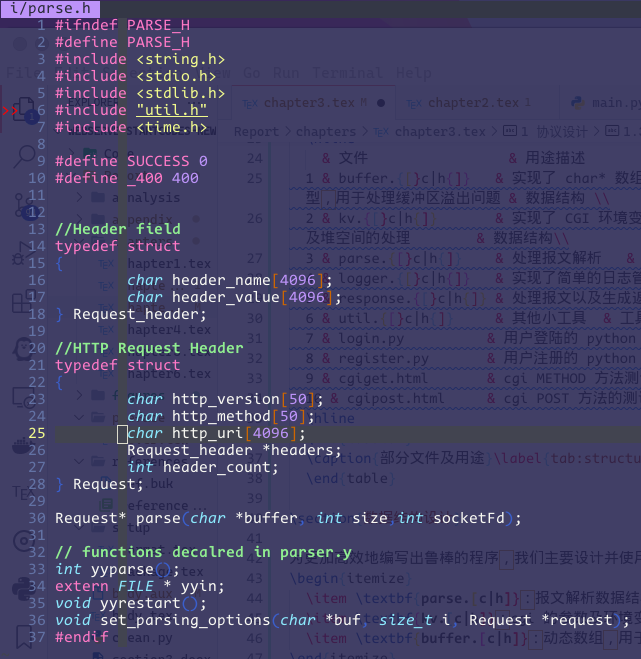
\includegraphics[width=1.6in]{parse.h.png}\label{fig:parse.h}}
  \subfigure[kv.h]{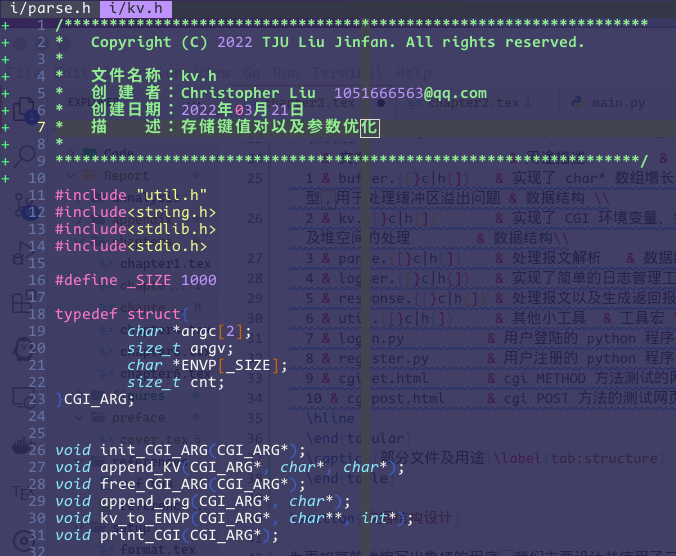
\includegraphics[width=2in]{kv.h.png}\label{fig:kv.h}}
  \subfigure[buffer.h]{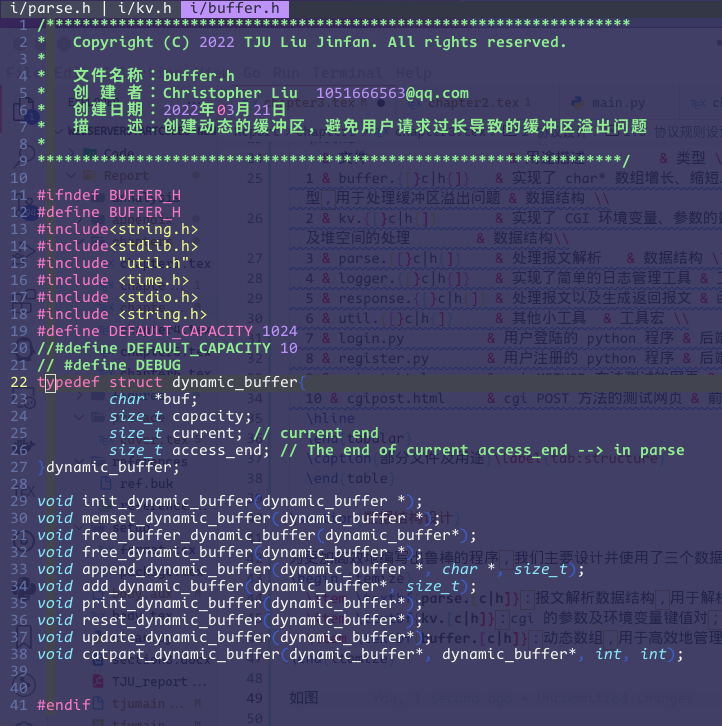
\includegraphics[width=1.65in]{buffer.h.png}\label{fig:buffer.h}}
  \caption{三个数据结构的原型}\label{fig:3datastructure}
\end{figure}

\section{协议规则设计}

以下将通过 socket 通信协议、消息解析协议、请求响应报文协议、流水线协议、多客户端并发请求协议以及CGI请求协议设计六个板块分别阐述 Liso server 运行的协议规则设计。

\subsection{使用 socket 进行网络通信的流程}

在本次实验中,我们通过使用 socket 套接字进行网络编程。socket 的功能,是提供一个统一的 API 使得应用程序在统一的框架下实现数据传输、数据接收等功能,使得编程人员能够更加专注于数据的处理以及算法,而非数据传输、接收这些模式统一的问题。

首先,我们对 socket 通信的流程进行说明。如图\ref{fig:socket1}所示,使用 socket 套接字收发报文的流程主要分为三大部分,分为是:初始化、收发数据以及关闭阶段

\begin{figure}
  \centering
  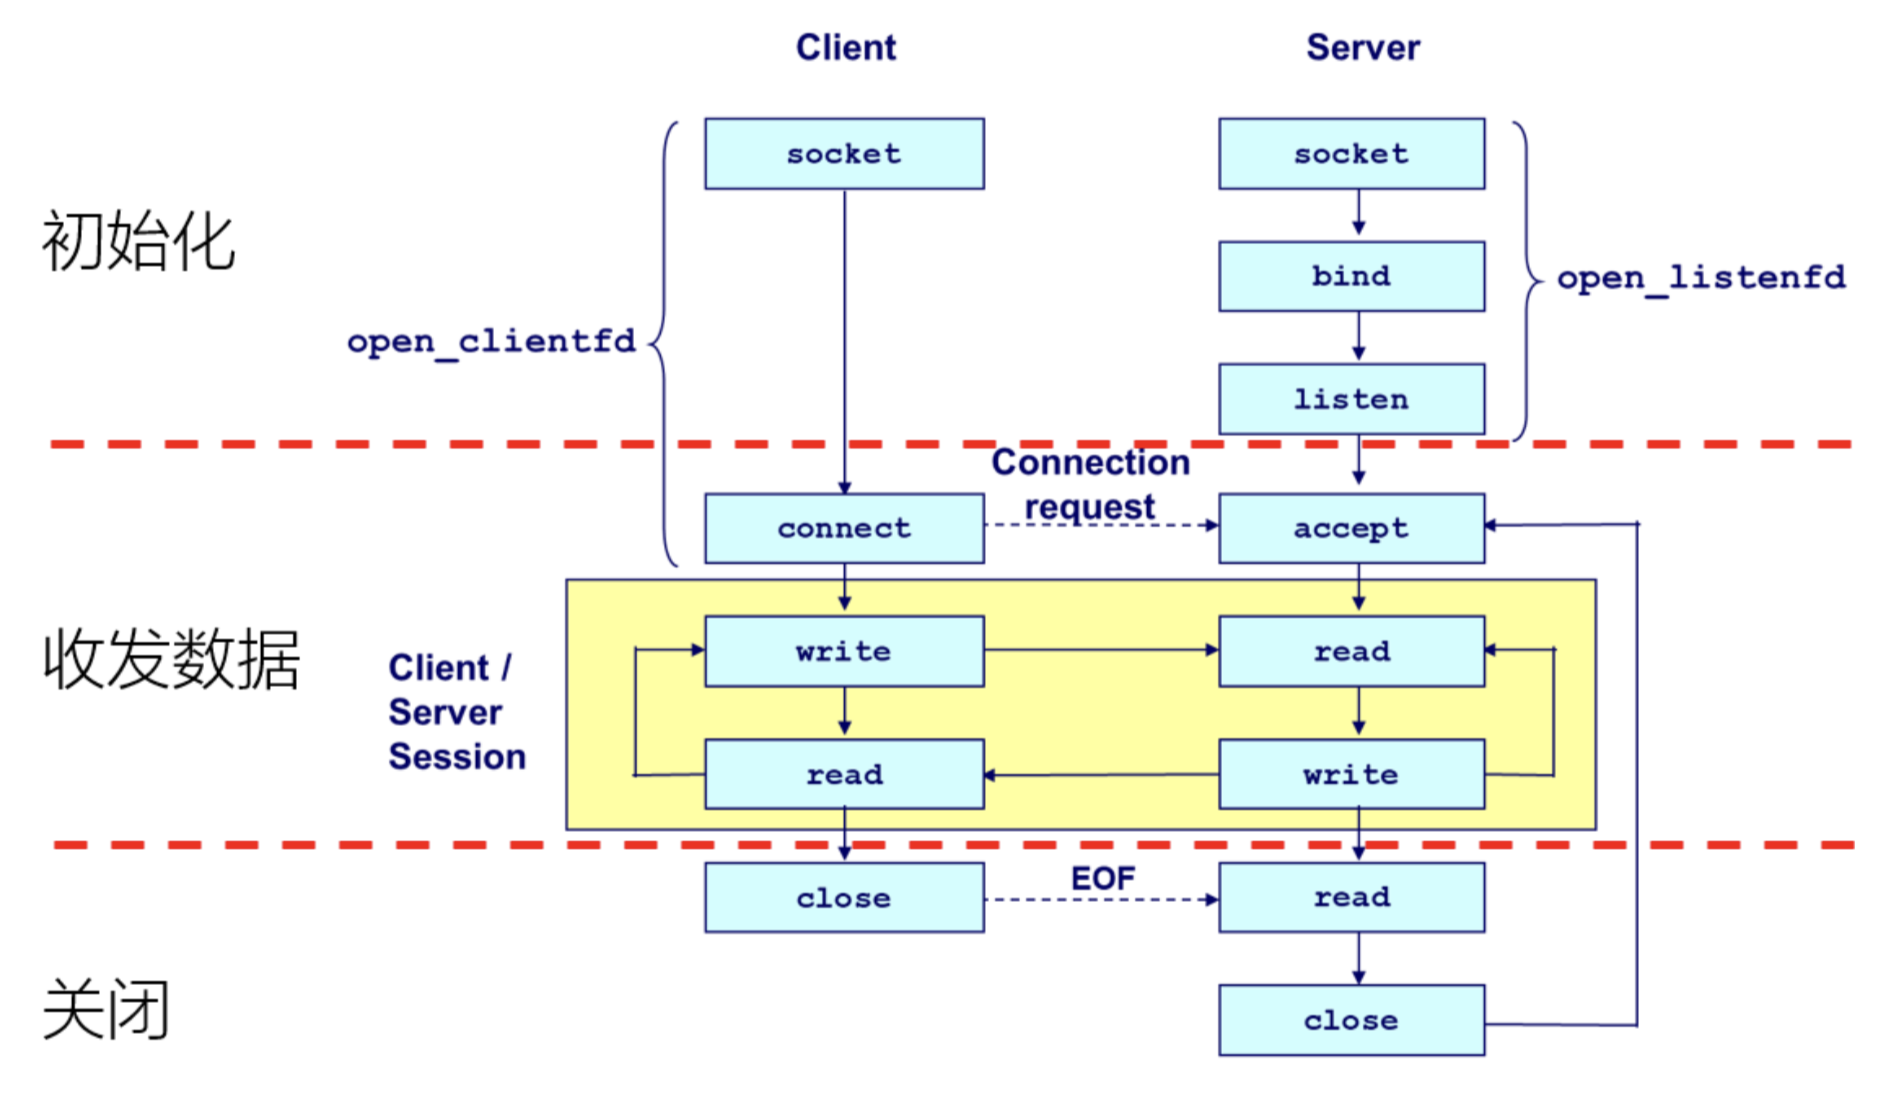
\includegraphics[width=5in]{socket_1.png}
  \caption{socket 编程流程图}\label{fig:socket1}
\end{figure}

\paragraph*{初始化阶段:} 客户端通过 socket 方法创建自己的网络位置(即 Ip 和 端口号);服务器创建 socket 之后还需要 bind 和进入 listen 状态,即监听有没有客户端发出与之互动的请求。

\paragraph*{收发阶段:} 客户端通过 connect 方法与远端主机的应用进程建立 TCP 连接,系统记录一个 socket 存储二者的 ip 及 端口号;在该阶段,服务器先通过 accept 函数获取一个连接请求,并为其分配一个服务端的文件描述符,作为 socket 表的索引。连接建立完成后,客户端和服务器就进入了“读、写”和“写、读”的循环当中。值的注意的是:在该过程中,客户端和服务端的“读、写”一定要是不对等的,即一方先读、一方先写,否则会出现竞争条件,产生死锁。在具体实现方面,客户端通过 socket 套接字将数据发送给服务端缓冲区内;服务端则通过解析模块对客户端的报文进行解析,并根据其请求方法,生成响应报文。最后,服务端将响应报文通过 socket 套接字放入缓冲区、发送给客户端。客户端再通过 socket 套接字得到服务端的响应报文。至此,一次完整的通信结束,如此循环往复,直到一方发出包含 “connection: close” 的请求, socket 最终关闭。

\paragraph*{关闭阶段:}当一方提出关闭时(如果支持了持久化连接,则通过“connection: close” 的头信息;否则默认只执行一次连接后就关闭 socket),结束通信,不得再发出任何报文, socket 被关闭。


\subsection{消息解析方法}

\paragraph*{Yacc 和 Lex 简介} 消息解析模块主要通过 lex 和 yacc 来实现。如图\ref{fig:yacclex} 所示,Lex 主要负责对字符串的模式进行识别,将其拆分成 token 并赋值给固定模式的变量(如图中的 id1, id2, id3 和 id4);Yacc 则对其中的关系进行运算,也就是在执行它的语法,如图中将固定模式的变量再次拆分成一颗运算树的结构。

\begin{figure}[htbp!]
  \centering
  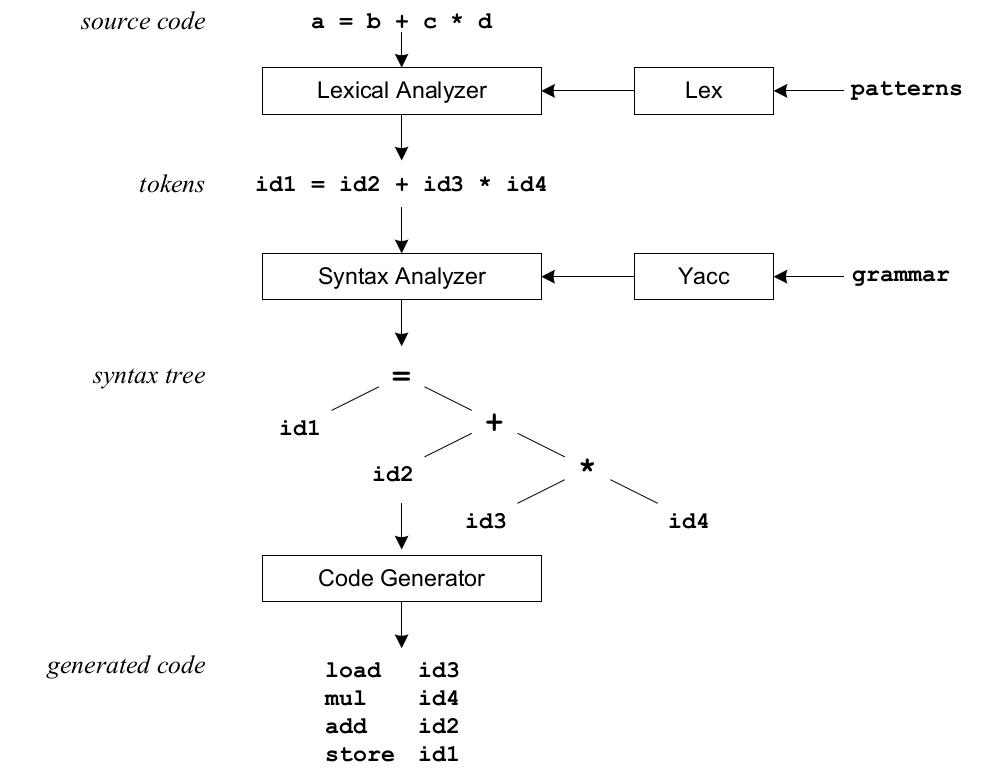
\includegraphics[width=5in]{yaccLex.png}
  \caption{yacc 和 lex 协同作用原理}\label{fig:yacclex}
\end{figure}

\paragraph*{实际应用} 在我们的程序中,lexer.l 定义了词法规则,例如 0\-9 就是 digit 等等的 token。而 parser.y 则定义了解析这些 token 的语法。例如以下的程序描述了一个关于请求头的语法定义,即一个请求开头,由 \{"token", "空格", "一段文字", "空格", "另一段文字", "换行符"\} 组成,且匹配到请求头时,要运行进行以下四行代码。

\begin{lstlisting}[language=c, name=parser.y Example]
request_line: token t_sp text t_sp text t_crlf {
  YPRINTF("request_Line:\n%s\n%s\n%s\n",$1, $3,$5);
  strcpy(parsing_request->http_method, $1);
  strcpy(parsing_request->http_uri, $3);
  strcpy(parsing_request->http_version, $5);
};
\end{lstlisting}

值的注意的是,yacc 支持一种递归定义的语法,让我们完成对多请求头语法的递归定义。如下代码即是示例。可以看到,1-12 行定义了基本的 request\_header,13行则循环定义了多条 request\_header 的语法。

\begin{lstlisting}[language=c, name=parser.y Example of Recursive Definition]
request_header: token ows t_colon ows text ows t_crlf {
  YPRINTF("request_Header:\n%s\n%s\n",$1,$5);
  strcpy(parsing_request->headers[parsing_request->header_count]
  .header_name, $1);
  strcpy(parsing_request->headers[parsing_request->header_count]
  .header_value, $5);
  parsing_request->headers = (Request_header *) realloc(
    parsing_request->headers, 
    (1+(++parsing_request->header_count)) * sizeof(Request_header)
    ); 
};

request_header: request_header request_header ;
\end{lstlisting}

至此,我们应当能够完成报文的解析,获得了相应的 header 键值对了。

\subsection{动态数组设计}

为了更方便、严谨地管理缓冲区以及返回信息等操作,我们编写了 buffer 工具。通过对堆内存的申请、操作、释放来控制流、字符串以及报文结构整理等操作。工具操作的函数在数据结构处已经描述过,主要是通过 malloc 和 realloc 来实现。

\subsection{请求报文与响应报文协议设计}

解析报文,只是我们服务端基础功能,接下来将以 GET 方法为例子,介绍基本的请求报文、响应报文的协议设计。在 client 端有如图\ref{fig:liso_client_get_test} 的运行效果。

\begin{figure}
  \centering
  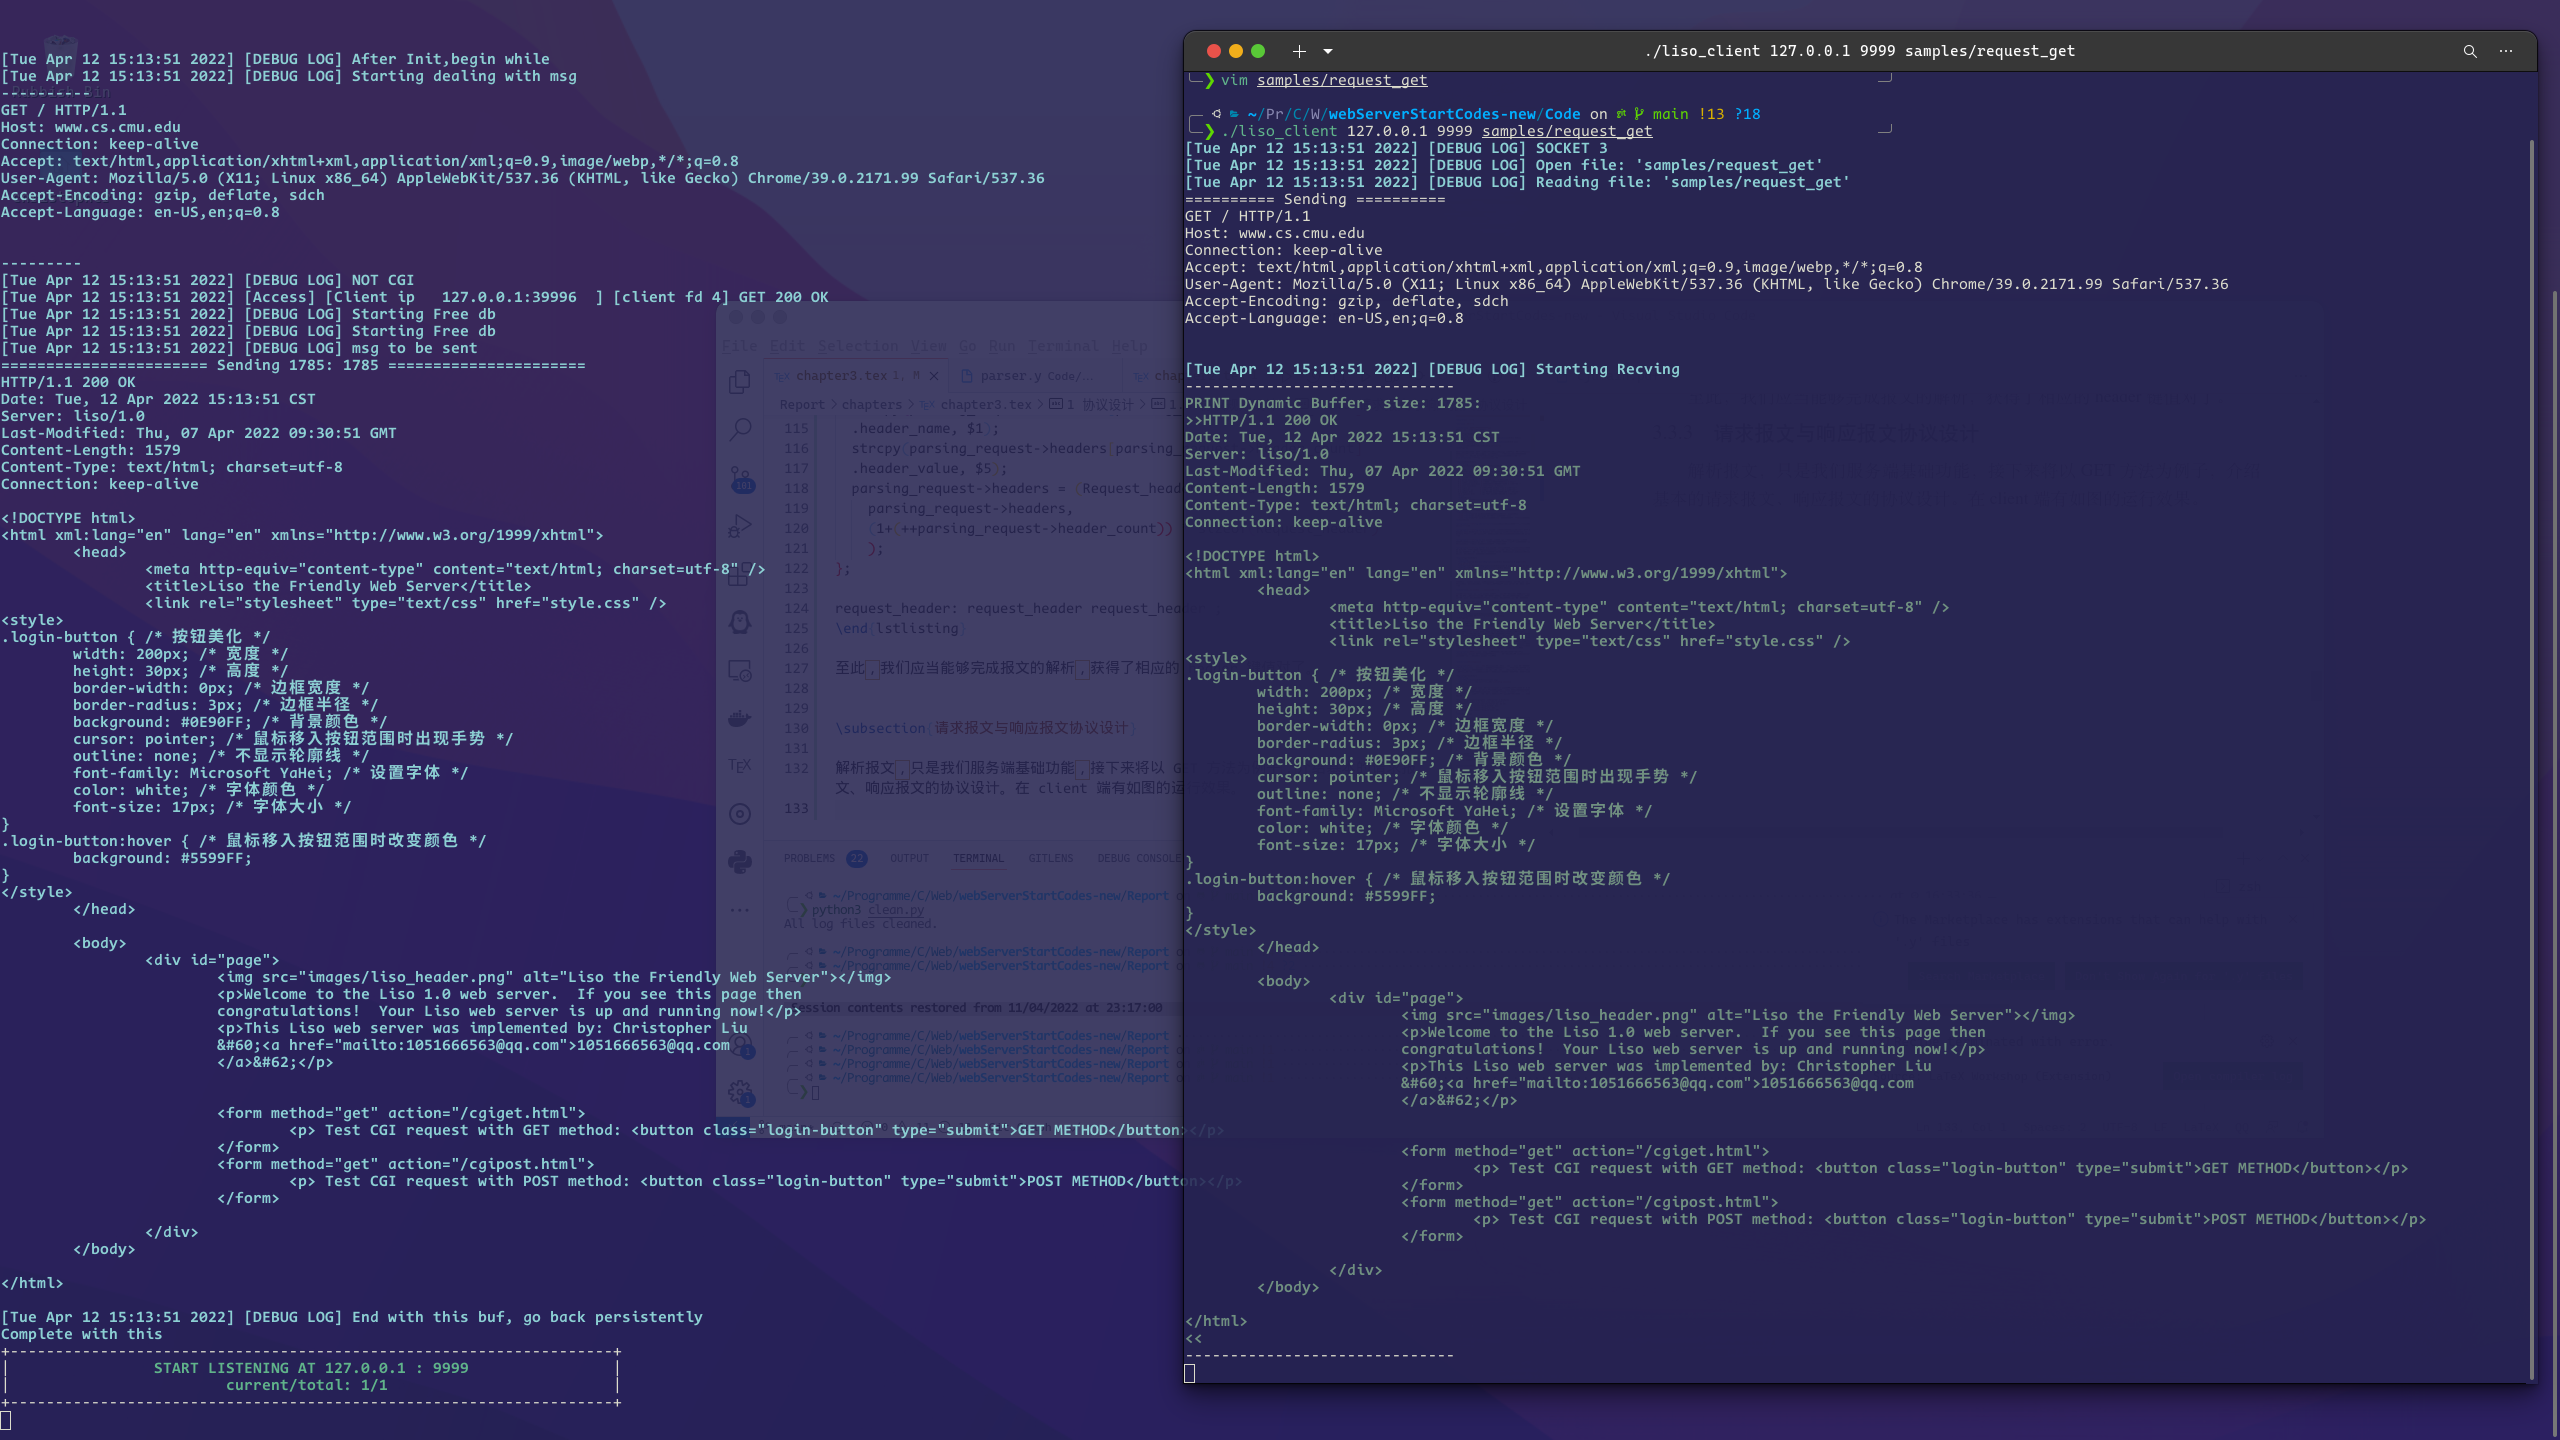
\includegraphics[width=5.5in]{liso_client_get_test.png}
  \caption{GET 请求测试}\label{fig:liso_client_get_test}
\end{figure}

第一行是的状态, "HTTP/1.1 200 OK",代表服务器的版本为 HTTP 1.1,状态码 200,状态信息 OK。对于服务器而言,只需在能够正确返回时将这些信息按顺序填入缓冲区即可。然后我们可以看到之后有 6 行键值对信息,即 \{"Date", "Server", "Last-Modified", "Content-Length", "Content-Type", "Connection"\},代表了\{"该请求的日期","服务器名称","最后编辑时间","Body 部分的长度","Body 部分数据的类型","连接状态"\}。同时,通过 Postman(一种后端即口测试工具,能够发送 HTTP 报文) 的测试,我们发现有些键值对并不是必须的,且顺序并不影响客户端收到正确的响应信息。当然,作为例子,我们将详细讲解这六个部分是如何得到并加入到响应报文中的。

\begin{itemize}
  \item \textbf{Date: } 通过 C 函数 time(),localtime() 以及 strftime() 将当前时间转化成一个字符串,然后通过统一函数调用 set\_header() 函数添加到响应报文的 headers 部分;
  \item \textbf{Server: } 服务器信息为完全一致的,不会因为请求的不同而有区别,故我们可以存放在宏中,使用时直接调用就可以了;
  \item \textbf{Last-Modified 等文件相关: } 标志着请求文件最近修改的时间,可以通过 stat() 函数得到;
  \item \textbf{Connection: } 一般来说不需要在意这个选项,只需设置为 keep-alive 就行,但我们考虑到做一些整体服务性能的优化,遇到错误的请求,就关闭这个连接,能够增加整体受到正确请求的概率,于是在受到错误请求时,将该选项设置为 close 否则就设置为缺省;
\end{itemize}

可以看到,在 Body 部分,我们加入了整个 HTML 文件,这是因为 GET 请求规则所致。所以如果是 HEAD 请求,我们就不会增加这个 Body 部分的内容。至于文件是如何加入到 Body 的,简单通过 mmap() 进行一个内存的映射即可,这个方法比 read() 更好的点在于不需要进行图片的特判而使用 fread() 等,mmap() 函数是通用的。唯一需要注意的是 mmap() 函数使用后还需要使用 munmap() 函数进行内存的释放,否则会出现 segment fault。


\subsection{流水线设计}

实现流水线作业的核心,在于从 Pipelining 的信息中拆分出单个报文。从 RFC2616 文档中得知其规则后,我们发现可以使用 "\textbackslash r\textbackslash n\textbackslash r\textbackslash n" 分割单个报文。所以我们通过 strstr() 函数,查出一个 "\textbackslash r\textbackslash n\textbackslash r\textbackslash n" 的位置,即是一个报文结尾处(严格来说还需要加上这个"\textbackslash r\textbackslash n\textbackslash r\textbackslash n" 才算结束)。

解析出一个报文后,我们通过自己实现的动态数组工具创建一个新的动态数组 newbuffer,然后通过函数 append\_dynamic\_buffer(),将报文加入到 newbuffer 中,然后通过设置 access\_end 记录当前报文在整个 pipelining 的位置。为什么要设计这个 access\_end 呢,因为在之后 cgi 中,可能会在 body 部分传输参数,然而这个 body 部分的内容会被 "\textbackslash r\textbackslash n\textbackslash r\textbackslash n" 拆分到下一条报文的开头,并不会添加到 newbuffer 中,也就是说我们只有在处理完一条报文之后才能确定该条报文的真实长度。为了统一性,我们才定义了这个 access\_end 结构体变量表示当前报文的结束位置。在完成该报文的所有工作之后,我们需要释放新创建的动态数组,并更新用来存放 pipelining 报文流的动态数组:通过函数 update\_dynamic\_buffer() 将 access\_end 前面的部分全部去掉。

这里需要注意的是,如果 body 部分未被接收完全,我们就开始对该报文进行处理时,我们需要正确返回,并回退到拆分报文之前的位置,待下一次接收后再处理该报文。


\subsection{多客户端并发处理协议}

对于多客户端并发访问,我们采用 select() 函数以及配套的 fd\_set 进行处理。核心思想是:通过 select() 函数监控有没有发出请求的客户端,然后通过他们的文件描述符判断是来发出 connection 请求还是收发数据,最后通过其接收的数据是否为0判断其是否离开。流程图如图\ref{fig:MultipleChart} 所示。

\begin{figure}[htbp!]
  \centering
  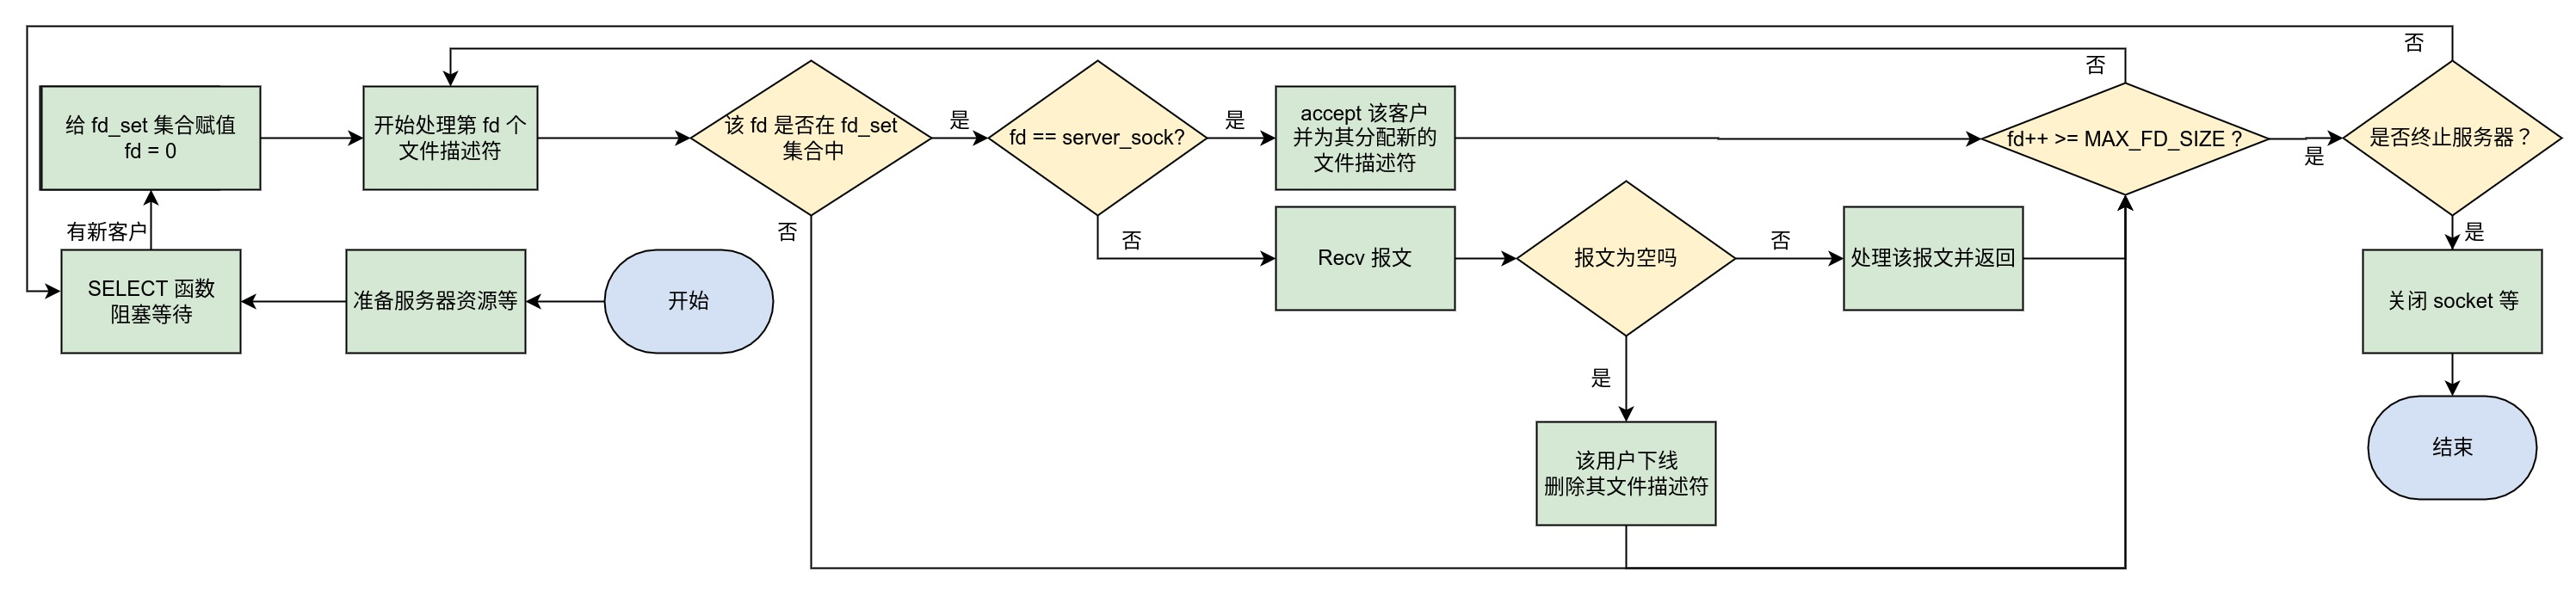
\includegraphics[width=5.6in]{FlowChart.jpg}
  \caption{多客户端并发流程图}\label{fig:MultipleChart}
\end{figure}

应该指出,我们通过 select() 函数,会得到一个用户池 fd\_set,之后只需要遍历该池的所有位置即可。需要注意的是,我们需要为每个用户预先开辟一个空的缓冲区,即 1024 个 dynamic\_buffer,来存放各自的数据。同时还需要维护每个用户的地址信息等。

\subsection{CGI 协议}\label{sec:CGI}

CGI 全称为 Common Gateway Interface,是实现服务器功能扩展的重要端口。其原理是:通过解析用户请求的 uri 是否含有 cgi 关键字,判断是否为 cgi 请求;如果是,则调用相应的 cgi 程序为其服务,否则按照正常情况处理。

根据实验指导书的意见,我们实现了如图的用户注册、登陆接口。在后端程序的编写中,我们采用了有良好跨平台性的 Python 以及 MySQL 数据库对用户信息进行存储,以便日后扩展时可以有良好的扩展接口。


CGI 实现的一般流程如下:
\begin{enumerate}
  \item 解析并处理该报文
  \item 判断 URI 中是否含有 cgi 的关键字(本次定义 /cgi/ 为关键字);
  \item 判断方法类型(仅支持 GET 和 POST);
  \item 判断请求参数是否完整(对于 POST 而言,可能尚未传输完成);
  \item 判断请求执行的文件是否存在、是否有权限执行;
  \item 执行请求执行的 CGI 脚本(或程序),并将输出数据贴在返回报文的 Body 部分;
  \item 按照正常的报文进行返回。
\end{enumerate}
